% Seminar 2 - Pagina 2 (continuare din pagina 1, 10-oct.-1994).
% Fragment pentru % Seminar 2 - Pagina 2 (continuare din pagina 1, 10-oct.-1994).
% Fragment pentru % Seminar 2 - Pagina 2 (continuare din pagina 1, 10-oct.-1994).
% Fragment pentru % Seminar 2 - Pagina 2 (continuare din pagina 1, 10-oct.-1994).
% Fragment pentru \input{seminars/pages/seminar2-pagina2-ro}; fără preambul.
% NOTE EDITORIALE:
% - Figura cu cele două mulţimi şi o retractă este o schemă desenată liber;
%   diagrama TikZ păstrează sensul, nu forma exactă a desenului.
% - În definiţia lui r, litera pentru unicul antecedent este citită ca u.
% - După "Fie f:A -> B" la exerciţiul 3 se află o abreviere neclară;
%   nu a fost completată prin presupunere.
% - Existenţa unei secţiuni pentru orice surjecţie foloseşte, în general,
%   axioma alegerii; manuscrisul alege câte un element din fiecare fibră,
%   fără să precizeze această ipoteză.
% - În figura de la punctul (c), proprietatea de epimorfism e indicată
%   prin două săgeţi paralele; nu am adăugat o demonstraţie inexistentă.

\subsection*{Seminar 2 - Pagina 2}

\noindent\fbox{$a\Rightarrow b$}\quad
\[
\begin{tikzcd}[column sep=large,row sep=small]
A \arrow[r,"f"] & B \arrow[d,"r"]\\
 & A
\end{tikzcd}
\qquad r(f(u))=u.
\]

% Schema din manuscris: mulţimile A şi B, imaginea lui f în B,
% şi o săgeată de întoarcere r: B -> A.
\begin{center}
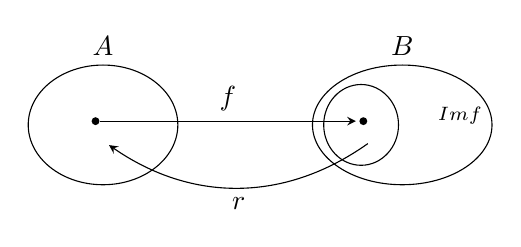
\begin{tikzpicture}[>=stealth,scale=.95]
  \draw (-2,0) ellipse (1.0 and .8);
  \draw (2,0) ellipse (1.2 and .8);
  \node at (-2,1.05) {$A$};
  \node at (2,1.05) {$B$};
  \draw (1.45,0) ellipse (.50 and .54);
  \node[font=\scriptsize] at (2.77,.13) {$\operatorname{Im}f$};
  \fill (-2.1,.05) circle (1.5pt);
  \fill (1.48,.05) circle (1.5pt);
  \draw[->] (-2.04,.05) -- (1.38,.05) node[midway,above] {$f$};
  \draw[->] (1.54,-.25) to[bend left=35] node[below] {$r$} (-1.92,-.27);
\end{tikzpicture}
\end{center}

\noindent Fie $a\in A$; definim
\[
r(y)=
\begin{cases}
u, & \text{dacă }f(u)=y,\\
a, & \text{dacă }y\notin\operatorname{Im}f.
\end{cases}
\]
\noindent Cum $f$ e inj., funcţia $r$ e corect definită.
\[
(r\circ f)(u)=r(f(u))=u
\quad\Longrightarrow\quad r\circ f=1_A.
\]

\medskip
\noindent\fbox{$b\Rightarrow a$}\quad
Fie $f(x_1)=f(x_2)$. Atunci
\[
r(f(x_1))=r(f(x_2))
\quad\Longrightarrow\quad x_1=x_2
\quad\Longrightarrow\quad f\text{ inj.}
\]

\medskip
\noindent\fbox{3}\quad Fie $f:A\longrightarrow B$.
\begin{enumerate}
\item[a)] $f$ surjectivă.
\item[b)] $f$ are o secţiune (există $s:B\longrightarrow A$ a.î.\ $f\circ s=1_B$).
\item[c)] $f$ este epimorfism:
\[
\begin{tikzcd}[column sep=large]
A \arrow[r,"f"] & B
\arrow[r,shift left=.55ex,"f_1"]
\arrow[r,shift right=.55ex,"f_2"'] & X
\end{tikzcd}
\]
\end{enumerate}

\noindent\underline{Sol.}

\noindent $a)\Rightarrow b)$.
\noindent $(\forall)\,y\in B$, $(\exists)\,x\in A$ a.î.\ $y=f(x)$.
\[
f^{-1}(y)=\{x\in A\mid f(x)=y\}\neq\varnothing.
\]
\noindent $(\forall)\,y\in B$, alegem $x_B\in f^{-1}(y)$ a.î.
\[
s(y)=x_B,\qquad (f\circ s)(y)=f(x_B)=y.
\]

\medskip
\noindent $b)\Rightarrow a)$.
\[
f\circ s\text{ surj.}\quad\Longrightarrow\quad f\text{ surj.}
\]
; fără preambul.
% NOTE EDITORIALE:
% - Figura cu cele două mulţimi şi o retractă este o schemă desenată liber;
%   diagrama TikZ păstrează sensul, nu forma exactă a desenului.
% - În definiţia lui r, litera pentru unicul antecedent este citită ca u.
% - După "Fie f:A -> B" la exerciţiul 3 se află o abreviere neclară;
%   nu a fost completată prin presupunere.
% - Existenţa unei secţiuni pentru orice surjecţie foloseşte, în general,
%   axioma alegerii; manuscrisul alege câte un element din fiecare fibră,
%   fără să precizeze această ipoteză.
% - În figura de la punctul (c), proprietatea de epimorfism e indicată
%   prin două săgeţi paralele; nu am adăugat o demonstraţie inexistentă.

\subsection*{Seminar 2 - Pagina 2}

\noindent\fbox{$a\Rightarrow b$}\quad
\[
\begin{tikzcd}[column sep=large,row sep=small]
A \arrow[r,"f"] & B \arrow[d,"r"]\\
 & A
\end{tikzcd}
\qquad r(f(u))=u.
\]

% Schema din manuscris: mulţimile A şi B, imaginea lui f în B,
% şi o săgeată de întoarcere r: B -> A.
\begin{center}
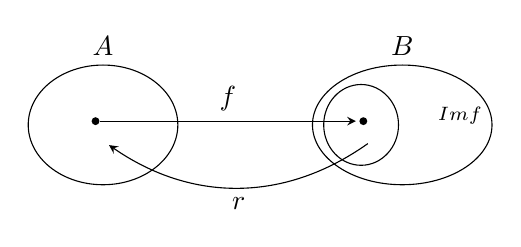
\begin{tikzpicture}[>=stealth,scale=.95]
  \draw (-2,0) ellipse (1.0 and .8);
  \draw (2,0) ellipse (1.2 and .8);
  \node at (-2,1.05) {$A$};
  \node at (2,1.05) {$B$};
  \draw (1.45,0) ellipse (.50 and .54);
  \node[font=\scriptsize] at (2.77,.13) {$\operatorname{Im}f$};
  \fill (-2.1,.05) circle (1.5pt);
  \fill (1.48,.05) circle (1.5pt);
  \draw[->] (-2.04,.05) -- (1.38,.05) node[midway,above] {$f$};
  \draw[->] (1.54,-.25) to[bend left=35] node[below] {$r$} (-1.92,-.27);
\end{tikzpicture}
\end{center}

\noindent Fie $a\in A$; definim
\[
r(y)=
\begin{cases}
u, & \text{dacă }f(u)=y,\\
a, & \text{dacă }y\notin\operatorname{Im}f.
\end{cases}
\]
\noindent Cum $f$ e inj., funcţia $r$ e corect definită.
\[
(r\circ f)(u)=r(f(u))=u
\quad\Longrightarrow\quad r\circ f=1_A.
\]

\medskip
\noindent\fbox{$b\Rightarrow a$}\quad
Fie $f(x_1)=f(x_2)$. Atunci
\[
r(f(x_1))=r(f(x_2))
\quad\Longrightarrow\quad x_1=x_2
\quad\Longrightarrow\quad f\text{ inj.}
\]

\medskip
\noindent\fbox{3}\quad Fie $f:A\longrightarrow B$.
\begin{enumerate}
\item[a)] $f$ surjectivă.
\item[b)] $f$ are o secţiune (există $s:B\longrightarrow A$ a.î.\ $f\circ s=1_B$).
\item[c)] $f$ este epimorfism:
\[
\begin{tikzcd}[column sep=large]
A \arrow[r,"f"] & B
\arrow[r,shift left=.55ex,"f_1"]
\arrow[r,shift right=.55ex,"f_2"'] & X
\end{tikzcd}
\]
\end{enumerate}

\noindent\underline{Sol.}

\noindent $a)\Rightarrow b)$.
\noindent $(\forall)\,y\in B$, $(\exists)\,x\in A$ a.î.\ $y=f(x)$.
\[
f^{-1}(y)=\{x\in A\mid f(x)=y\}\neq\varnothing.
\]
\noindent $(\forall)\,y\in B$, alegem $x_B\in f^{-1}(y)$ a.î.
\[
s(y)=x_B,\qquad (f\circ s)(y)=f(x_B)=y.
\]

\medskip
\noindent $b)\Rightarrow a)$.
\[
f\circ s\text{ surj.}\quad\Longrightarrow\quad f\text{ surj.}
\]
; fără preambul.
% NOTE EDITORIALE:
% - Figura cu cele două mulţimi şi o retractă este o schemă desenată liber;
%   diagrama TikZ păstrează sensul, nu forma exactă a desenului.
% - În definiţia lui r, litera pentru unicul antecedent este citită ca u.
% - După "Fie f:A -> B" la exerciţiul 3 se află o abreviere neclară;
%   nu a fost completată prin presupunere.
% - Existenţa unei secţiuni pentru orice surjecţie foloseşte, în general,
%   axioma alegerii; manuscrisul alege câte un element din fiecare fibră,
%   fără să precizeze această ipoteză.
% - În figura de la punctul (c), proprietatea de epimorfism e indicată
%   prin două săgeţi paralele; nu am adăugat o demonstraţie inexistentă.

\subsection*{Seminar 2 - Pagina 2}

\noindent\fbox{$a\Rightarrow b$}\quad
\[
\begin{tikzcd}[column sep=large,row sep=small]
A \arrow[r,"f"] & B \arrow[d,"r"]\\
 & A
\end{tikzcd}
\qquad r(f(u))=u.
\]

% Schema din manuscris: mulţimile A şi B, imaginea lui f în B,
% şi o săgeată de întoarcere r: B -> A.
\begin{center}
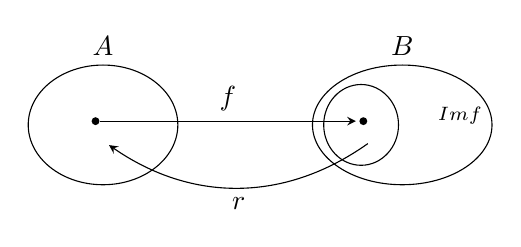
\begin{tikzpicture}[>=stealth,scale=.95]
  \draw (-2,0) ellipse (1.0 and .8);
  \draw (2,0) ellipse (1.2 and .8);
  \node at (-2,1.05) {$A$};
  \node at (2,1.05) {$B$};
  \draw (1.45,0) ellipse (.50 and .54);
  \node[font=\scriptsize] at (2.77,.13) {$\operatorname{Im}f$};
  \fill (-2.1,.05) circle (1.5pt);
  \fill (1.48,.05) circle (1.5pt);
  \draw[->] (-2.04,.05) -- (1.38,.05) node[midway,above] {$f$};
  \draw[->] (1.54,-.25) to[bend left=35] node[below] {$r$} (-1.92,-.27);
\end{tikzpicture}
\end{center}

\noindent Fie $a\in A$; definim
\[
r(y)=
\begin{cases}
u, & \text{dacă }f(u)=y,\\
a, & \text{dacă }y\notin\operatorname{Im}f.
\end{cases}
\]
\noindent Cum $f$ e inj., funcţia $r$ e corect definită.
\[
(r\circ f)(u)=r(f(u))=u
\quad\Longrightarrow\quad r\circ f=1_A.
\]

\medskip
\noindent\fbox{$b\Rightarrow a$}\quad
Fie $f(x_1)=f(x_2)$. Atunci
\[
r(f(x_1))=r(f(x_2))
\quad\Longrightarrow\quad x_1=x_2
\quad\Longrightarrow\quad f\text{ inj.}
\]

\medskip
\noindent\fbox{3}\quad Fie $f:A\longrightarrow B$.
\begin{enumerate}
\item[a)] $f$ surjectivă.
\item[b)] $f$ are o secţiune (există $s:B\longrightarrow A$ a.î.\ $f\circ s=1_B$).
\item[c)] $f$ este epimorfism:
\[
\begin{tikzcd}[column sep=large]
A \arrow[r,"f"] & B
\arrow[r,shift left=.55ex,"f_1"]
\arrow[r,shift right=.55ex,"f_2"'] & X
\end{tikzcd}
\]
\end{enumerate}

\noindent\underline{Sol.}

\noindent $a)\Rightarrow b)$.
\noindent $(\forall)\,y\in B$, $(\exists)\,x\in A$ a.î.\ $y=f(x)$.
\[
f^{-1}(y)=\{x\in A\mid f(x)=y\}\neq\varnothing.
\]
\noindent $(\forall)\,y\in B$, alegem $x_B\in f^{-1}(y)$ a.î.
\[
s(y)=x_B,\qquad (f\circ s)(y)=f(x_B)=y.
\]

\medskip
\noindent $b)\Rightarrow a)$.
\[
f\circ s\text{ surj.}\quad\Longrightarrow\quad f\text{ surj.}
\]
; fără preambul.
% NOTE EDITORIALE:
% - Figura cu cele două mulţimi şi o retractă este o schemă desenată liber;
%   diagrama TikZ păstrează sensul, nu forma exactă a desenului.
% - În definiţia lui r, litera pentru unicul antecedent este citită ca u.
% - După "Fie f:A -> B" la exerciţiul 3 se află o abreviere neclară;
%   nu a fost completată prin presupunere.
% - Existenţa unei secţiuni pentru orice surjecţie foloseşte, în general,
%   axioma alegerii; manuscrisul alege câte un element din fiecare fibră,
%   fără să precizeze această ipoteză.
% - În figura de la punctul (c), proprietatea de epimorfism e indicată
%   prin două săgeţi paralele; nu am adăugat o demonstraţie inexistentă.

\subsection*{Seminar 2 - Pagina 2}

\noindent\fbox{$a\Rightarrow b$}\quad
\[
\begin{tikzcd}[column sep=large,row sep=small]
A \arrow[r,"f"] & B \arrow[d,"r"]\\
 & A
\end{tikzcd}
\qquad r(f(u))=u.
\]

% Schema din manuscris: mulţimile A şi B, imaginea lui f în B,
% şi o săgeată de întoarcere r: B -> A.
\begin{center}
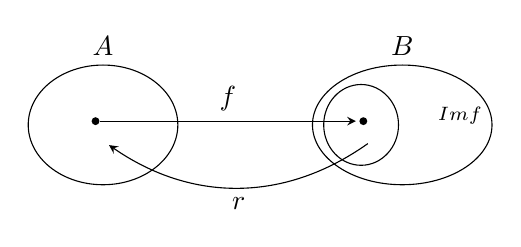
\begin{tikzpicture}[>=stealth,scale=.95]
  \draw (-2,0) ellipse (1.0 and .8);
  \draw (2,0) ellipse (1.2 and .8);
  \node at (-2,1.05) {$A$};
  \node at (2,1.05) {$B$};
  \draw (1.45,0) ellipse (.50 and .54);
  \node[font=\scriptsize] at (2.77,.13) {$\operatorname{Im}f$};
  \fill (-2.1,.05) circle (1.5pt);
  \fill (1.48,.05) circle (1.5pt);
  \draw[->] (-2.04,.05) -- (1.38,.05) node[midway,above] {$f$};
  \draw[->] (1.54,-.25) to[bend left=35] node[below] {$r$} (-1.92,-.27);
\end{tikzpicture}
\end{center}

\noindent Fie $a\in A$; definim
\[
r(y)=
\begin{cases}
u, & \text{dacă }f(u)=y,\\
a, & \text{dacă }y\notin\operatorname{Im}f.
\end{cases}
\]
\noindent Cum $f$ e inj., funcţia $r$ e corect definită.
\[
(r\circ f)(u)=r(f(u))=u
\quad\Longrightarrow\quad r\circ f=1_A.
\]

\medskip
\noindent\fbox{$b\Rightarrow a$}\quad
Fie $f(x_1)=f(x_2)$. Atunci
\[
r(f(x_1))=r(f(x_2))
\quad\Longrightarrow\quad x_1=x_2
\quad\Longrightarrow\quad f\text{ inj.}
\]

\medskip
\noindent\fbox{3}\quad Fie $f:A\longrightarrow B$.
\begin{enumerate}
\item[a)] $f$ surjectivă.
\item[b)] $f$ are o secţiune (există $s:B\longrightarrow A$ a.î.\ $f\circ s=1_B$).
\item[c)] $f$ este epimorfism:
\[
\begin{tikzcd}[column sep=large]
A \arrow[r,"f"] & B
\arrow[r,shift left=.55ex,"f_1"]
\arrow[r,shift right=.55ex,"f_2"'] & X
\end{tikzcd}
\]
\end{enumerate}

\noindent\underline{Sol.}

\noindent $a)\Rightarrow b)$.
\noindent $(\forall)\,y\in B$, $(\exists)\,x\in A$ a.î.\ $y=f(x)$.
\[
f^{-1}(y)=\{x\in A\mid f(x)=y\}\neq\varnothing.
\]
\noindent $(\forall)\,y\in B$, alegem $x_B\in f^{-1}(y)$ a.î.
\[
s(y)=x_B,\qquad (f\circ s)(y)=f(x_B)=y.
\]

\medskip
\noindent $b)\Rightarrow a)$.
\[
f\circ s\text{ surj.}\quad\Longrightarrow\quad f\text{ surj.}
\]
